\chapter{Results}
\textit{In this chapter the results on behalf of the data analysis will be shown. A paired t-test of the mean magnitude for each frequency band specified in \ref{sec:...} is computed to test the significance level of the difference for the uncuffed and cuffed conditions.}

\section{Paired t-test}
To test if there is a statistical significant difference between the uncuffed and cuffed condition a paired t-test is applied on the outcome data from the data analysis. The approach builds on using the total mean of each frequency band, condensing these down to just one number for each frequency band for one ROI for one subject. 

Before a paired t-test is calculated for the data, a boxplot is computed to get a visual representation of the data of the three frequency bands. The boxplots can be seen in \figref{fig:boxEndo} throughout \figref{fig:boxMyo}. 

\begin{figure}[H]
	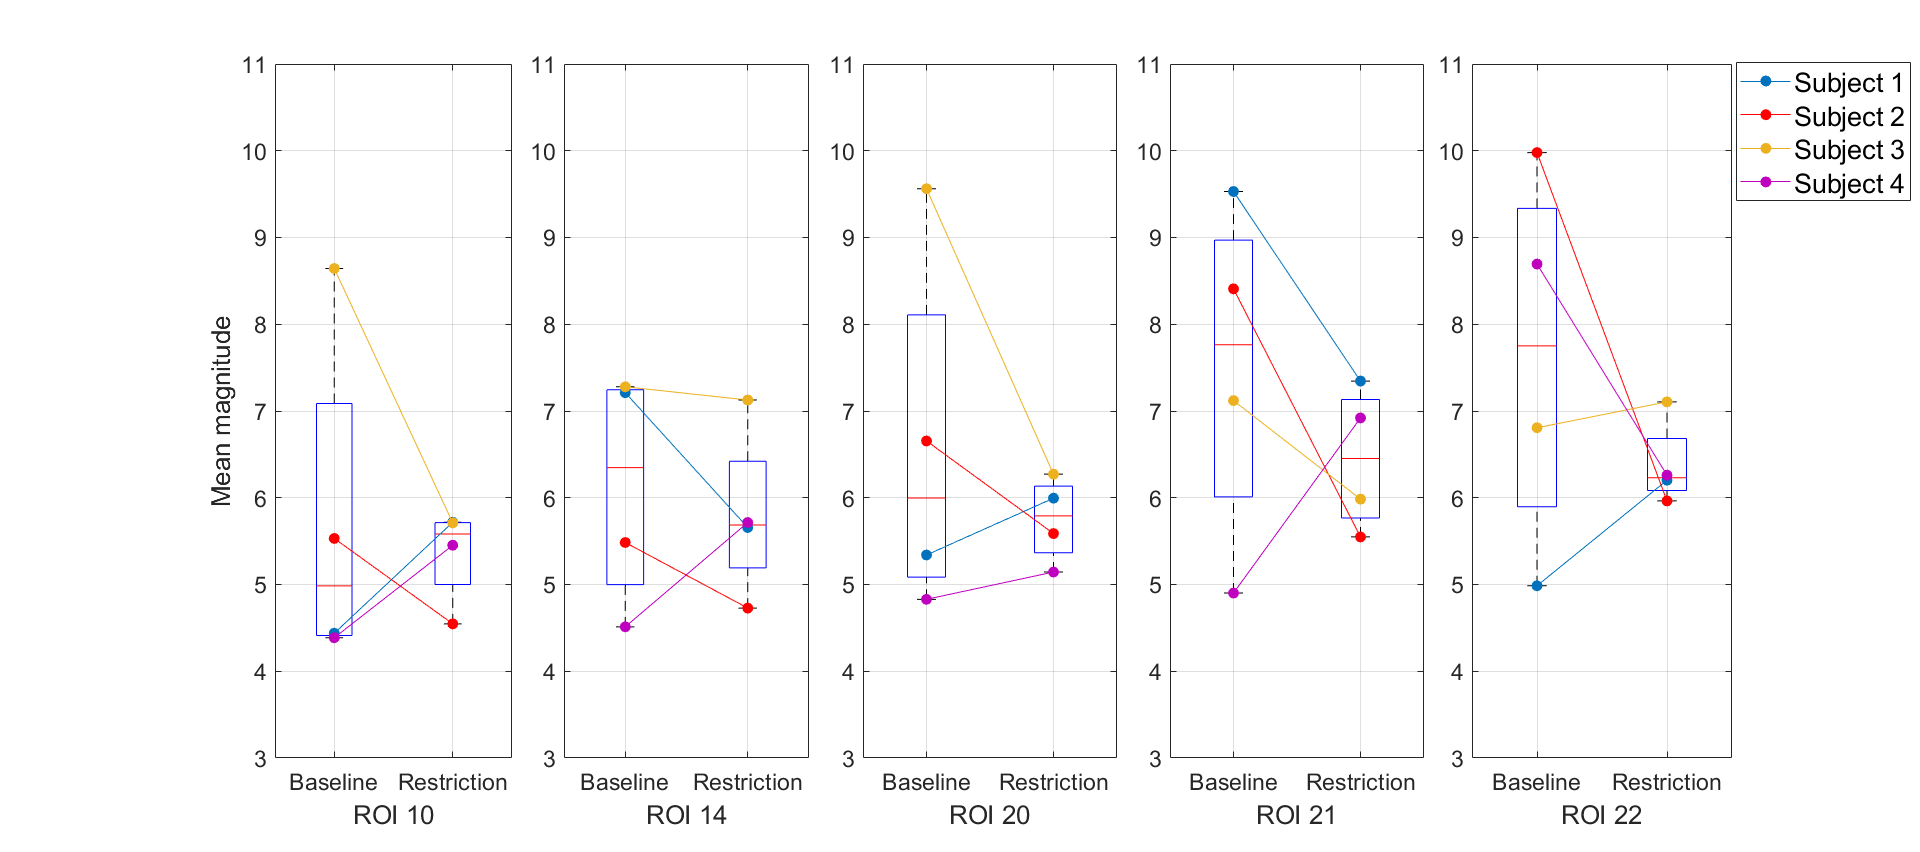
\includegraphics[width=1\textwidth]{figures/boxplot_endo}
	\caption{Boxplot for mean magnitude for the endothelial frequency band, for uncuffed versus cuffed in five ROI.}
	\label{fig:boxEndo}
\end{figure}

\begin{figure}[H]
	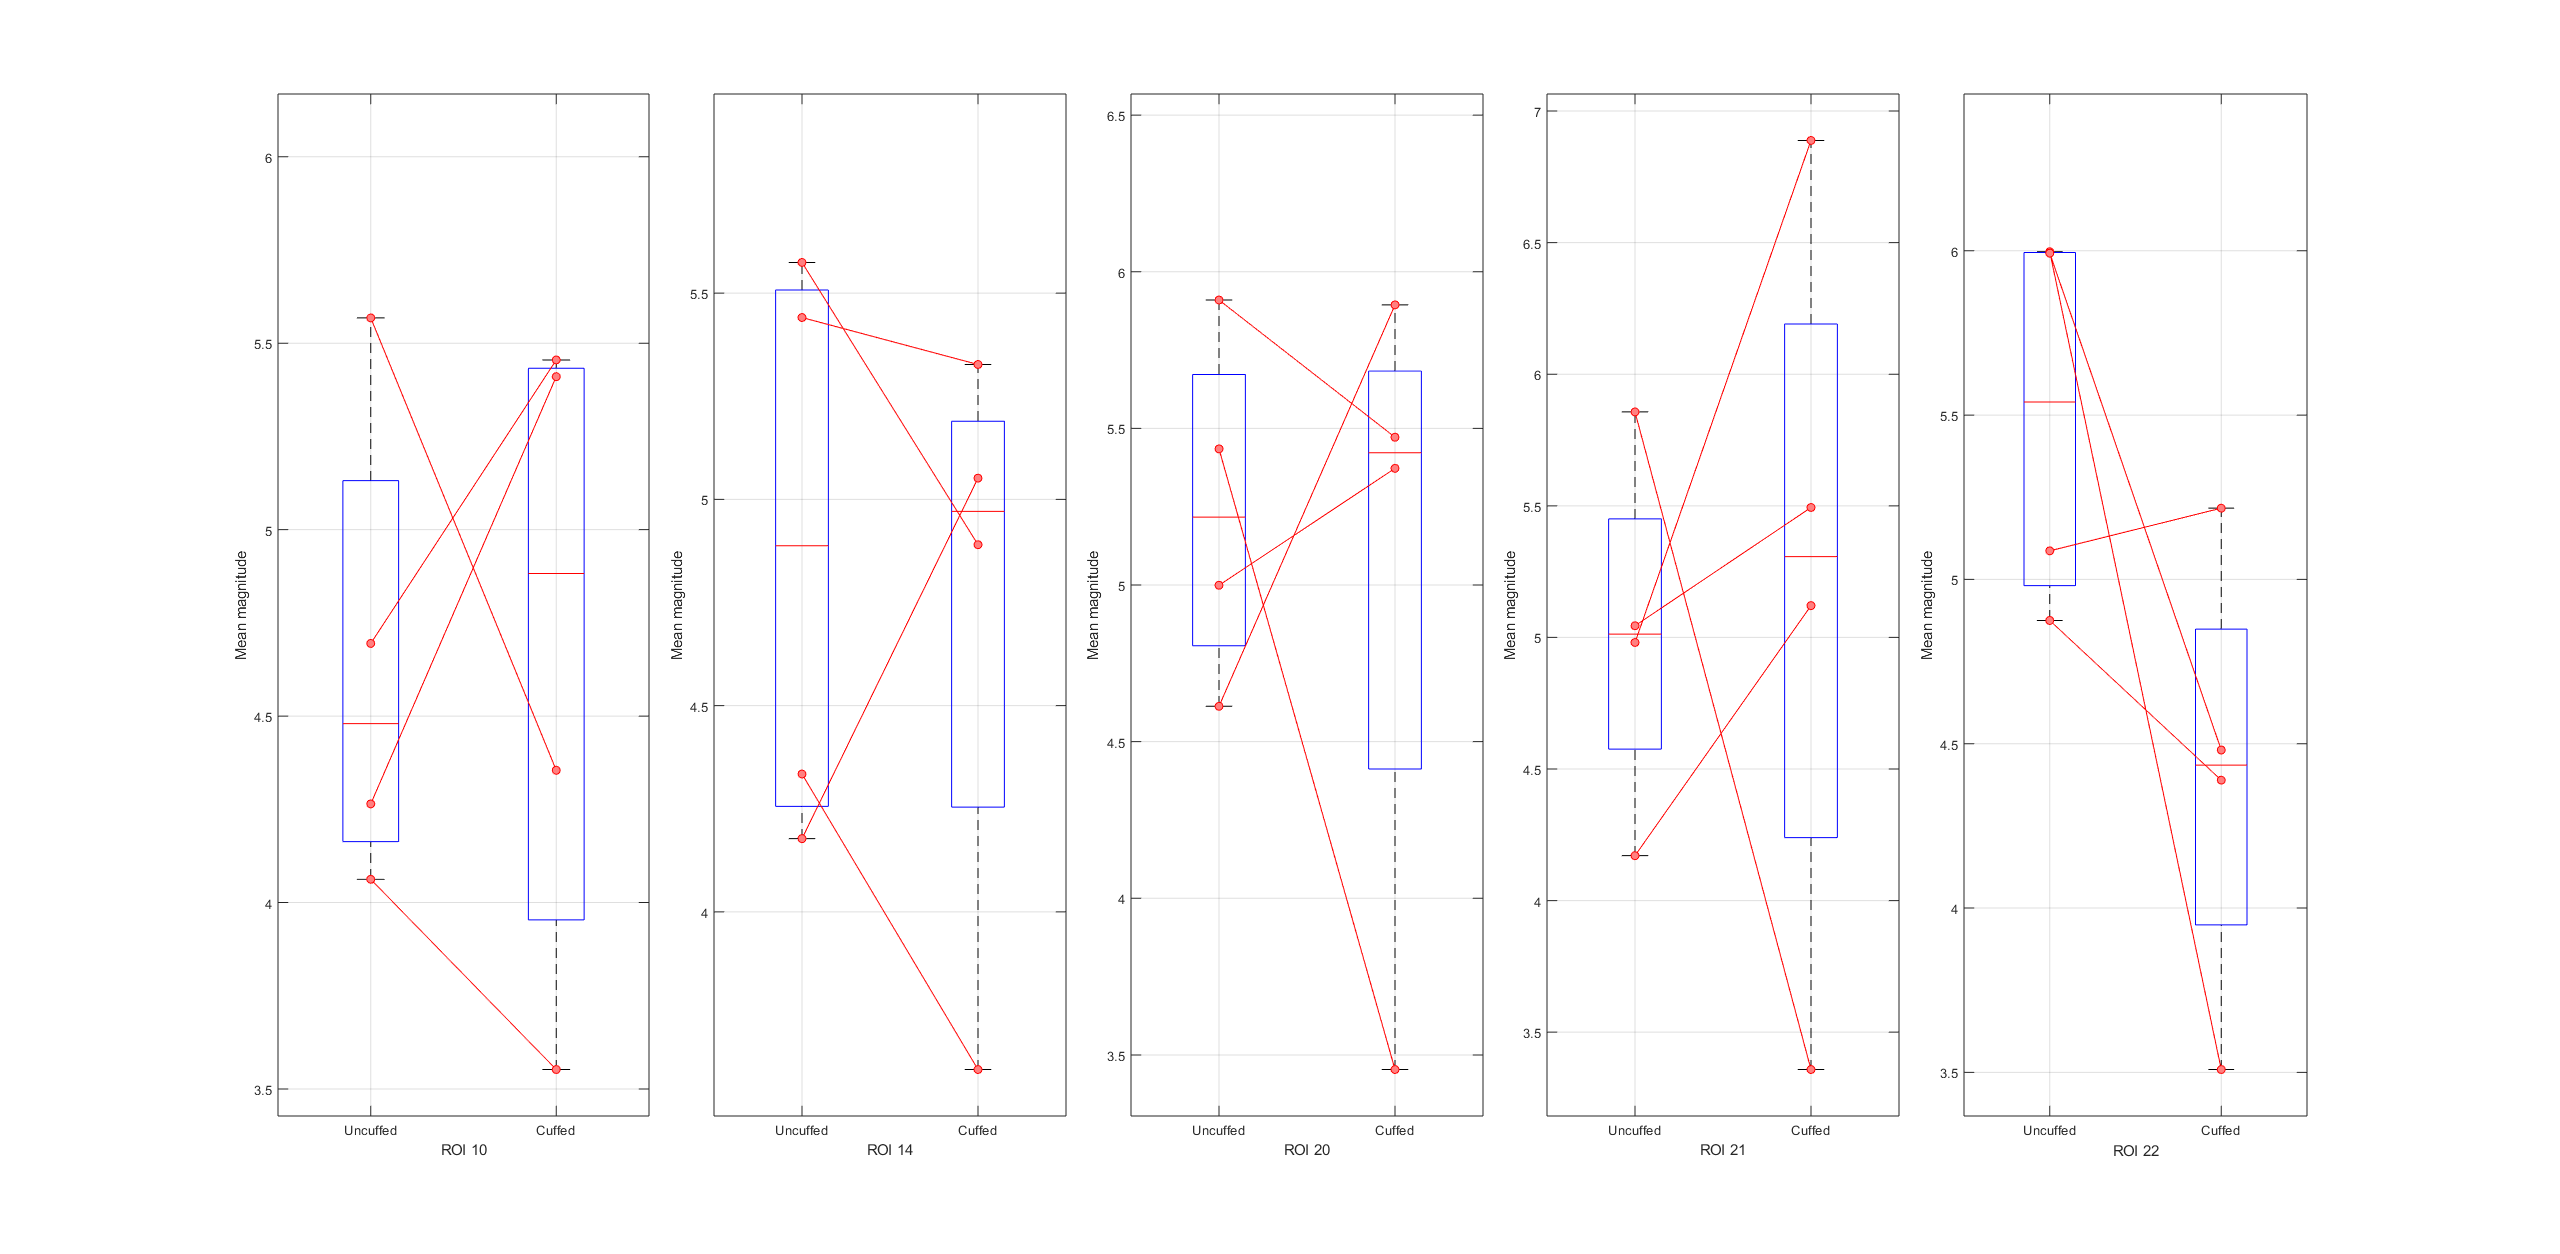
\includegraphics[width=1\textwidth]{figures/boxplot_neuro}
	\caption{Boxplot for mean magnitude for the neurogenic frequency band, for uncuffed versus cuffed in five ROI.}
	\label{fig:boxNeuro}
\end{figure}

\begin{figure}[H]
	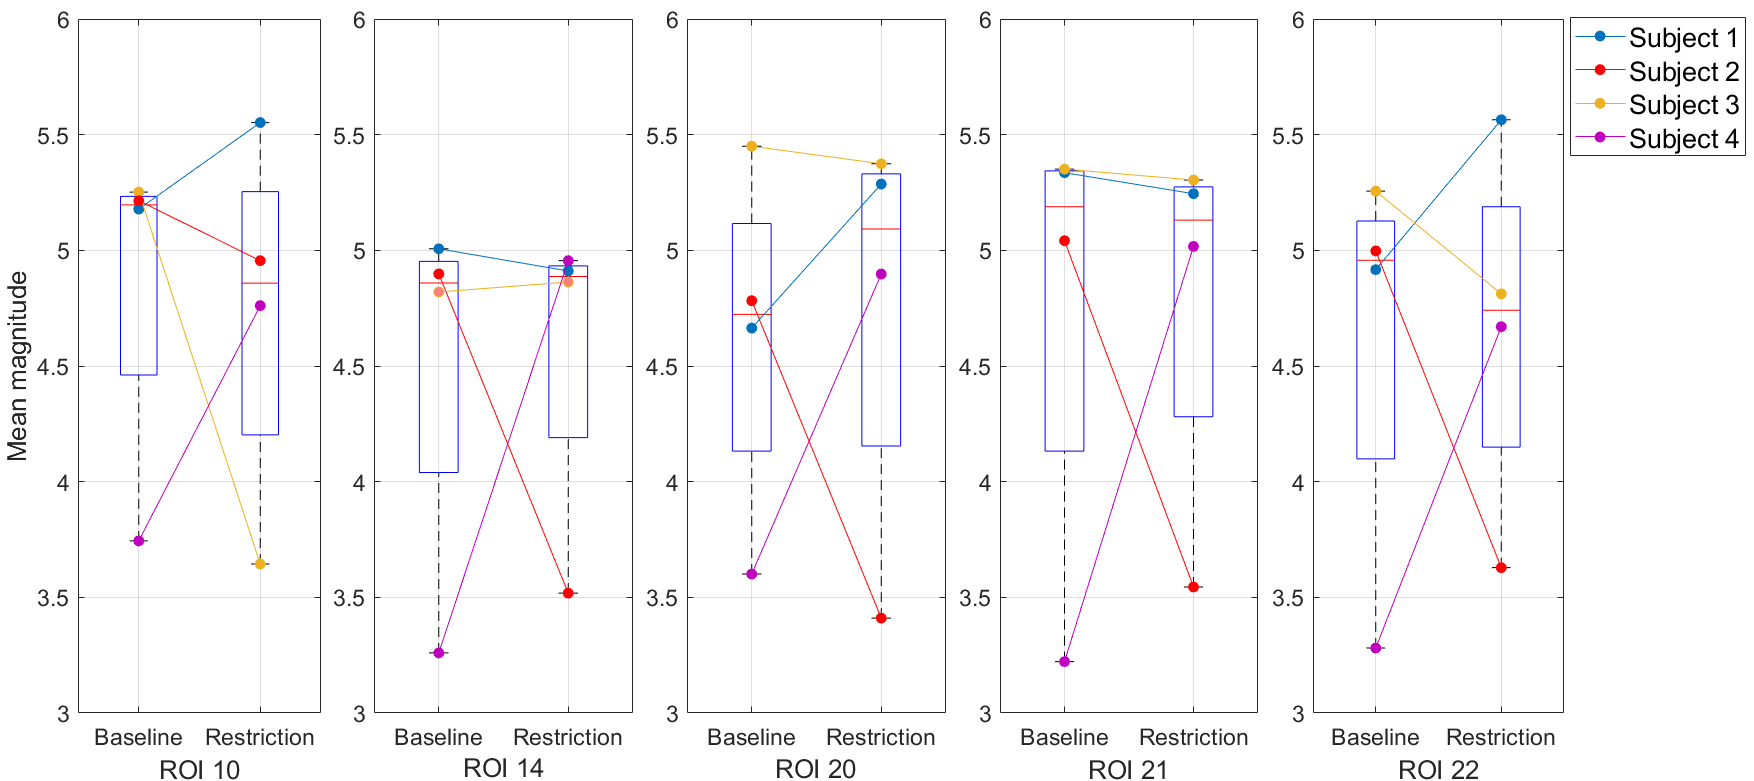
\includegraphics[width=1\textwidth]{figures/boxplot_myo}
	\caption{Boxplot for mean magnitude for the myogenic frequency band, for uncuffed versus cuffed in five ROI.}
	\label{fig:boxMyo}
\end{figure}

The boxplots show points for each mean of the magnitude, a line is connecting the before and after condition to indicate if there has been an increase or decrease in magnitude. A paired t-test will be performed on all five regions, where uncuffed is the before condition and cuffed is the after condition. The outcome of the paired t-test will either be rejecting the h0 hypothesis, that there is no difference between the two conditions, or not rejecting the h0 hypothesis, which indicates that there is a difference.
 
%In the paired t-test none of the data from the frequency bands show a significant difference between subject in cuffed and uncuffed condition. 
A table showing the p-values of the statistical test is shown in \ref{my:pval}. 
\begin{table}[H]
	\centering
	\scalebox{0.8}{
	\begin{tabular}{|l|l|l|l|}
		\hline
		& \textbf{P-endo} & \textbf{P-myo}  & \textbf{P-neuro} \\ \hline
		\textbf{ROI 10} & 0.7116 & 0.8454 & 0.9389  \\ \hline
		\textbf{ROI 14} & 0.6254 & 0.9237 & 0.6955  \\ \hline
		\textbf{ROI 20} & 0.4141 & 0.9237 & 0.8004  \\ \hline
		\textbf{ROI 21} & 0.4062 & 0.9564 & 0.8452  \\ \hline
		\textbf{ROI 22} & 0.3826 & 0.9323 & 0.1552  \\ \hline
	\end{tabular}}
\caption{Table showing the p-values corresponding to specific ROI in correlation with frequency band.}
	\label{my:pval}
\end{table}
As indicated in table \ref{my:pval}, all of the tests show a significance level well above 0.005. %The lowest p-value is presented in region 22 where a p-value of 0.1552 for the neurogenic band is found. 
When reflecting the p-values onto the boxplots it can easily be seen the correlation between the p-values and the occurrence of a difference in the dataset. 
  
%\section{T-value mapping}
%Results illustrated on \figref{fig:black}, shows a t-value mapped image from a summation of each subjects scalogram within the two conditions. The y-axis shows the number of different frequencies and the x-axis is time, giving in number of frames. Each pixel within the image has a t-value corresponding to the test of the uncuffed pixel value compared to the cuffed pixel value. The larger t-value, the brighter a pixel will appear in the image. The image showed no areas where a greater difference could be observed. Mostly individual pixels lid up showing a great difference, but as these are individual and not part of an area, these are considered outliers.  

%\begin{figure}[H]
%	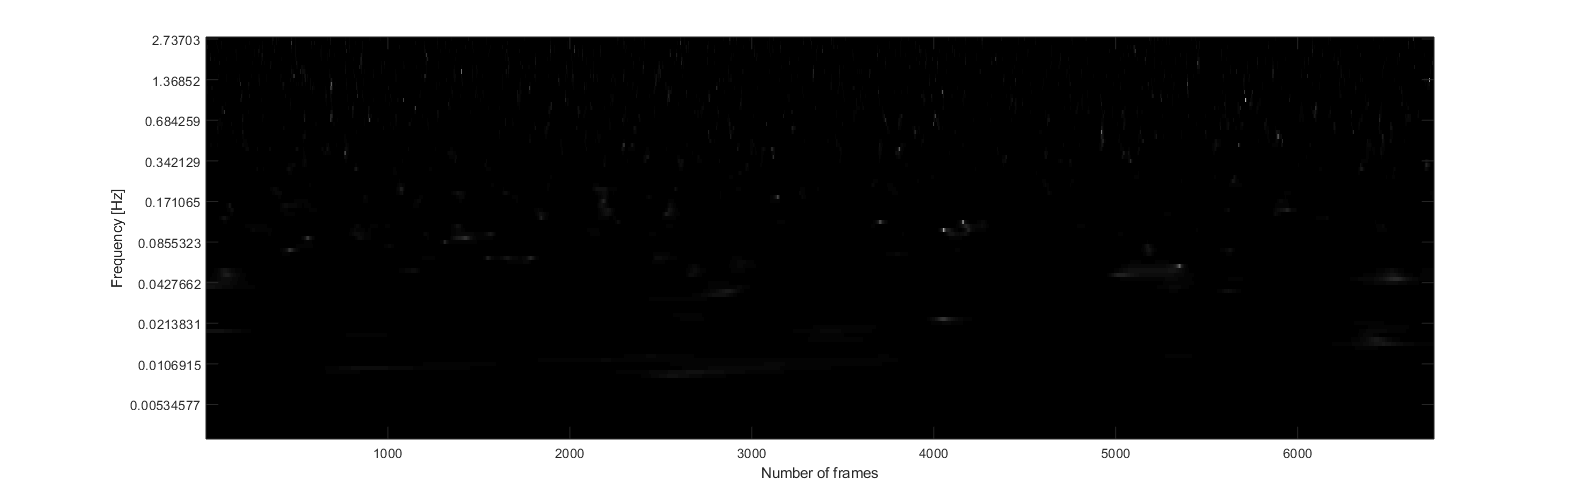
\includegraphics[width=1\textwidth]{figures/t-values_roi10}
%	\caption{t-value mapped image, from a t-test of region 10, uncuffed versus cuffed.}
%	\label{fig:black}
%\end{figure}

%Neither of the images corresponding to each region showed areas where vasomotion activity could be identified. The remaining t-value mapping images can be seen in \cref{t-value}.  
%The number of positive and negative t-values for each frequency band in every region is compared in \cref{tab:t}. Positive t-values indicate a drop in amplitude from the uncuffed state to the cuffed and negative values the opposite. No  
%\begin{table}[H]
%	\centering
%	\caption{Table with comparison of t-values for every band at every region.}
%	\label{tab:t}
%	\scalebox{0.7}{
%	\begin{tabular}{|l|l|l|l|}
%		\hline
%		& Endo band      & Neuro band     & Myo band       \\ \hline
%		\multicolumn{4}{|l|}{Region 10}                                         \\ \hline
%		Positive vs negative & 76377 vs 65352 & 49665 vs 38072 & 55092 vs 52892 \\ \hline
%		\multicolumn{4}{|l|}{Region 20}                                         \\ \hline
%		Positive vs negative & 79309 vs 62428 & 44248 vs 43489 & 52116 vs 55968 \\ \hline
%		\multicolumn{4}{|l|}{Region 21}                                         \\ \hline
%		Positive vs negative & 74634 vs 67095 & 43542 vs 44195 & 52941 vs 55043 \\ \hline
%		\multicolumn{4}{|l|}{Region 22}                                         \\ \hline
%		Positive vs negative & 88601 vs 53128 & 64195 vs 23542 & 51462 vs 56522 \\ \hline
%	\end{tabular}}
%\end{table}
%T is simply the calculated difference represented in units of standard error. The greater the magnitude of T (it can be either positive or negative), the greater the evidence against the null hypothesis that there is no significant difference. The closer T is to 0, the more likely there isn't a significant difference.

%\section{ANOVA}